\documentclass[a4paper,11pt]{article}
\usepackage[finnish]{babel}

\usepackage{amsmath}
\usepackage[utf8]{inputenc}
\usepackage[T1]{fontenc}
\usepackage{parskip}
\usepackage{csquotes}
\usepackage{graphicx}
\usepackage{epstopdf}

\usepackage{amsmath}
\usepackage{amssymb}
\usepackage{eurosym}
\usepackage{tyyli}

\usepackage[backend=biber,style=numeric]{biblatex}
\addbibresource{viitteet.bib}

\begin{document}

{
\thispagestyle{empty}
{\large
\textbf{Helsingin yliopisto}
\par
MAST31901 - History of Mathematics
}

\vspace{7cm}

{\huge
Kurssiessee:}
\par
{\Large \bf Euler ja lukuteoria}

\vspace{2cm}

{\Large Elli Kiiski}

\vfill

{\large \today}
}

\clearpage

\pagenumbering{arabic}

\section{Johdanto}

On hankala päättää millä titteleillä hänet esittelisi; ainoastaan hänen ansioluettelonsa läpikäyminen vaatisi oman kymmensivuisen esseensä. Tällä kertaa tarkoitusperiimme kuitenkin sopii tituleerata tätä yleisneroa matemaatikko Leonhard Euleriksi.

Määrittelyongelmat eivät tosin jää siihen, sillä Euler onnistui tuottamaan mullistavia tuloksia myös ällistyttävän monella eri osa-alueella matematiikan alan sisällä. Poistamme hetkeksi mielestämme maailman kauneimman yhtälön\footnote{Eulerin identiteettiä $e^{\pi i}+1=0$ on verrattu Shakespearin sonettin ja testattu maailman kauneimmaksi yhtätlöksi jopa magneettikuvaustutkimuksilla! \cite{identity}} sekä Königsbergin siltaongelman\footnote{Euler todisti, ettei Königsbergissä (nykyinen Kaliningrad) ollut mahdollista tehdä kävelyretkeä, jolla ylittää kunkin kaupungin seitsemästä sillasta täsmälleen kerran \cite{silta}} ja keskitymme tällä erää matematiikan kuningattareen\footnote{\enquote{Mathematics is the queen of the sciences and number theory is the queen of mathematics.}\\Carl Friedrich Gauss \cite{quotes}}, lukuteoriaan. Eulerin saavutukset yksin tällä sektorilla olisivat varmasti riittäneet nostamaan hänet historiankirjoihin yhtenä historian suurimmista matemaatikoista.

Yhtäläisesti historiallisena kuin matemaattisenakin esseenä tasapainottelemme näiden näkökulmien välillä varoen uppoutumasta liian syvällisesti kumpaankaan. Toisaalta pyrkimyksenä on koota yhteen johdonmukainen kuva Eulerin lukuteoreettisesta elämäntyöstä niin ajallisessa kuin matemaattisessakin kontekstissa. Se kaikki alkaa jo hyvän aikaa ennen Eulerin syntymää.

\section{Lukuteoria ennen Euleria}
\label{kakkoi}

Oikeastaan vielä Eulerinkaan aikana ei puhuttu matematiikan alasta nimeltä lukuteoria \cite{Karatsuba}. Kuitenkin ongelmia, joiden katsotaan nykyään kuuluvan lukuteorian piiriin, on ratkottu paljon ennen ajanlaskumme alkua. Ensimmäisenä todisteena pidetään babylonialaista Plimpton 322 savitaulua, joka sisältää vaikuttavan määrän yhtälön $a^2+b^2=c^2$ toteuttavia lukukolmikoita, joita kutsutaan tätä nykyä Pythagoraan kolmikoiksi.

Juuri Pythagoraan (n. 580–500 eaa.) nimissä olevat löydökset, joihin kuuluu noiden kolmikoiden ja niihin liittyvän Pythagoraan lauseen lisäksi mm. monikulmioluvut kuten kolmio- ja neliöluvut, ovat ensimmäisiä merkkejä lukujen teoreettisemmasta tutkimisesta \cite{Burton}. Myös myöhemmin tutuksi tulevat täydelliset luvut (\textit{perfect number}) ja ystävälliset lukuparit (\textit{amicable numbers}) yhdistetään häneen ja aikalaisiin seuraajiinsa.

Antiikin kreikan toinen suuri matemaatikko Euklides (n. 300 eaa.) tunnetaan etenkin vaikuttavasta teoksessaan \textit{Elements} \cite{Elements}, joka käsittelee pääosin geometriaa. Sen kirjoissa VII ja IX esitellään kuitenkin perustavanlaatuisia lukuteorian tuloksia etenkin alkulukuihin liittyen. Merkittävimpiin poimintoihin kuuluvat mm. Euklideen algoritmi (suurimman yhteisen tekijän löytäminen) ja todistus alkulukujen määrän äärettömyydestä. Euklides todisti myös Eulerin myöhemmin täydentämän lauseen

\begin{center}
    \textit{Jos luku $a$ on muotoa $(2^p-1)2^{p-1}$, missä sekä $p$ että $2p-1$ ovat alkulukuja, $a$ on täydellinen (määritellään luvussa \ref{kolmoi}).}
\end{center}

Diophantes tässä välissä jos se on wörtti mainita vielä

Tässä välissä oli taas taukoa ettei paljon kiinnostanut, kunnes tuli

Pierre de Fermat (1601–1665) 

Vuonna XXXX syntyi Leonhard Euler, joka seuraavana YY elinvuotenaan kehitti eteenpäin (lähes) jokaisen aikaansa edeltäneen lukuteoreetikon aikaansaannoksia.

\section{Täydelliset luvut ja ystävälliset parit}
\label{kolmoi}

Kuten todettu, tuottoisana matemaatikkona Euler ehti tuottaa lukuisia löytöjä ja todistuksia myös lukuteorian saralla. Vaikka monimutkaisimmat näistä saavat n. vuoden matematikaan opiskelijankin raapimaan päätään, osa puolestaan vaikuttaa nykyihmiselle hyvinkin yksinkertaisilta. Kansantajuisimmasta päästä ovat niin kutsutut täydelliset luvut ja ystävälliset lukuparit.

\begin{center}
    \textbf{Täydellinen luku} \textit{Positiivinen kokonaisluku, joka on omien itseään pienempien tekijöidensä summa. \textit{Esimerkiksi} luku $6$ on täydellinen, koska $1+2+3=6$.}
\end{center}

Palataan nyt aiemmin luvussa \ref{kakkoi} esiteltyyn Euklideen täydellisiä lukuja koskevaan lauseeseen, jolle Euler todisti omana aikanaan vahvemman version, joka kuuluu näin

\begin{center}
    \textit{Jos luku $a$ on parillinen täydellinen luku se voidaan kirjoittaa muodossa $(2^p-1)2^{p-1}$, missä sekä $p$ että $2p-1$ ovat alkulukuja.}
\end{center}

Euler siis näytti, että Euklideen todistama yhteys täydelliseten lukujen ja lausekkeen $(2^p-1)2^{p-1}$ välillä pätee myös toiseen suuntaan. Siinä missä Euklides näytti, että luvun toteuttaessa kyseisen lausekkeen, se on täydellinen, Euler osoitti, että luvun ollessa täydellinen ja parillinen (parittomia täydellisiä lukuja ei ole löydetty tai niiden olemassaolemattomuutta todistettu \ref{lähde}) se toteuttaa kyseisen lausekkeen.

Ystävälliset lukuparit liittyvät läheisesti täydellisiin lukuihin, tavallaan tällaisten lukujen voisi luonnehtia olevan ikään kuin täydellisiä toisilleen. Täsmällinen määritelmä kuuluu seuraavasti:

\begin{center}
    \textbf{Ystävällinen lukupari} \textit{Pari $(A, B)$ erisuuria positiivisia kokonaislukuja, joille pätee, että luvun $A$ itseään pienempien tekijöiden summa on $B$ sekä toisinpäin. \textit{Esimerkiksi} $(220, 284)$ on tällainen.}
\end{center}

Ennen Euleria ystävällisiä lukupareja oli löydetty vasta kaksi, niin kutsutut Pythagoraan pari $(220, 284)$ sekä Fermat-Descartesin pari $(17296, 18416)$. Eulen kasvatti tätä määrää huimalla 59 parilla, joiden joukossa on myös parittomia lukupareja. Esimerkiksi $(67095=3^3\cdot5\cdot7\cdot71, 71145=3^3\cdot5\cdot17\cdot31)$ on Eulerin löytämä pariton ystävällinen lukupari.

Ystävällisiä lukupareja tunnetaan nykyään yli miljardi, joista pisimmät ovat tuhansia numeroita pitkiä. Tietokoneiden laskentatehon kehityksellä on tietenkin ollut tähän valtava vaikutus, ja uusien löytöjen algoritmista generointia voi tuskin verrata Eulerilla käytössään olleisiin metodeihin. Tutkimalla lukujen ominaisuuksia Euler kuitenkin huomasi alkuluvuilla olevan hyödyllisiä ominaisuuksia tekijöiden summia laskettaessa, joita hän pystyi käyttämään hyväkseen. \cite{tarvii kaivaa siitä yhdestä exam paperista}

Loppujen lopuksi onkin vähemmän merkittävää, kuinka monta uutta ystävällistä lukuparia tai täydellistä lukua Euler itse onnistui löytämään. Hänen kehittämänsä menetelmät niiden tuottamiseen sen sijaan ovat antaneet työkaluja tulevaisuuden matemaatikoille kasvattaa kyseisiä lukulistoja.

\section{Eulerin $\varphi$-funktio ja muita nimikkotuotteet}

Siltä varalta, ettei Eulerin massiivista aikaansannosten määrää ole vielä alleviivattu tarpeeksi, päästään kyseiseen tavoitteeseen viimeistään tutkimalla Wikipedia-sivua \textit{List of things named after Leonhard Euler} (lista Leonhard Eulerin mukaan nimetyistä asioista) \cite{listofthings}. Eulerin identiteetti vilahti jo erässä alaviitteessä, mutta listaus sisältää tietysti myös useita merkittäviä lukuterian tuloksia.

Eulerin $\varphi$-funktio (\textit{engl. Euler's totient function}) on eräs lukuteoriassa usein näyttäytyvistä (ja ehkä myös yksi kiinnostavimmista\footnote{Esseen kirjoittaja sattui tekemään kandityönsä \textit{The Order of Euler's totient function} kyseisen funktion kasvuvauhdin alarajasta \cite{kandi}}) funktioista. Sen arvo kertoo lukujen jaollisuudesta, tosin käänteisesti: mitä useammalla luvulla jaollinen luku on, sitä pienempi on suhteessa $\phi$-funktion arvo.

\begin{center}
    \textbf{Eulerin $\phi$-funktio $\phi: \N \rightarrow \N$}\\
    \textit{$\phi(1)=1$ sekä kaikilla $n\geq2$, $\phi(n)$ on sellaisten lukujen $1,2,...,n$ määrä, joiden suurin yhteinen tekijä luvun $n$ kanssa on $1$.}
\end{center}

Myöhemmin käsiteltävien tulosten lisäksi $\phi$-funktiota käytetään myös MISSÄ.

Lukuteorian Eulerin vakio nönön, ei pidä sekoittaa:  Myös luonnollisen logaritmin kantaluku $e\approx2,71823$, vaikkakin suomenkieliseltä nimeltään Neperin luku, on nimetty löytäjänsä Eulerin mukaan.



\section{Fermatin töille jatkoa}

Fermat, Eulerin lähin edeltäjä??, jonka työt olivat hyvin tuttuja hänelle. Euler kumosi osan Fermatin uumoiluista ja todisti osan ja generalisoi osan.

Fn keissi kumosi

Generalisoi fermatin pienen lauseen (tarvii fii funktion tähän apuun)



\section{Eulerin perintö}

Konjektuuri, ettei ole parittomia alkulukuja (ei vieläkän todistettu)

\section{muistiinpanot}

\subsection{A. A. Karatsuba}

In Euler’s time there was no such a field of science as “number theory.” s.1

Yleisti euklideen lauseen täydellisista luvuista (mersenne prime) ja löysi 59 amicable number pairia (kohta 1)

Frematin konjektuuri että Fn on kaikki alkulukuja, Euler disproves (kohta 2a)

Yleisti fermatin pienen teoreeman fii-funktion avulla (kohta 2b)

Kongruenssin ja quadratic residues, Legendre-juttuja en muista mitään mutta Euler muototoili quadratic reciprocityn mutta ei vielä todistanut (kohta 2c)

Lukujen esittäminen $x^2+y^2$ jne muodossa, Euler todisti luvuille muotoa 4n+1 jne. (kohta 2d)

Pellin yhtälön ja continued fractions yhdistävä alkgoritmi jotenki en ihan tajuu (kohta 2e)

Jotain neljän neliön summa Lagrangen kanssa ja että kuinka lähelle lukua voi päästä kahden neliön summalla, ilmeisesti jatkoa kohtaan 2d (kohta 2f)

Todisti fremat's last theorem kun n=3, sen innoittamana(?) syntyi algbraic number theory (kohta 2gg)

Euler keppas  primitive roots and indices (kohta 3)

Keksi idean transkendenttiluvuista (kohta 4)

Löytyy aina ailkuluku välistä n ja 2n, f(x) = x2 - x+ A antaa alkulukuja, Goldbach problem (kohta 5)

Euler is the author of two methods for solving problems in number theory by means of analysis mut ei kerrota mitkä??? (kohta 6)

Euler ja Bach ??? (kohta 7)

Euler's identity ja Reiamnnin zeta funktio, voi käyttää apuna todistamaan infinitely many primes, myös Dirichlet characters ja Dirichlet’s
L-function ja Chebyshev’s studies of 1848, joista en ymmärtänyt ensilukemalla mitään OKEI tää kohta pitää lukee paremmilla aivoilla uudestaan jos on tarpeellinen (kohta 8)

loput meni ihan yli hilseen (kohta 9)

\subsection{random}

Wikipedian teoreemalistauksessa 9kpl missä Eulerin nimi

Pitäis varmaan lukee oma kandi taas



\section{Eulerin elämä}

Leonhard Euler on yksi kaikkien aikojen tunnetuimmista matemaatikoista ja hänet tunnetaan mone jahas

\begin{figure}
    \centering
    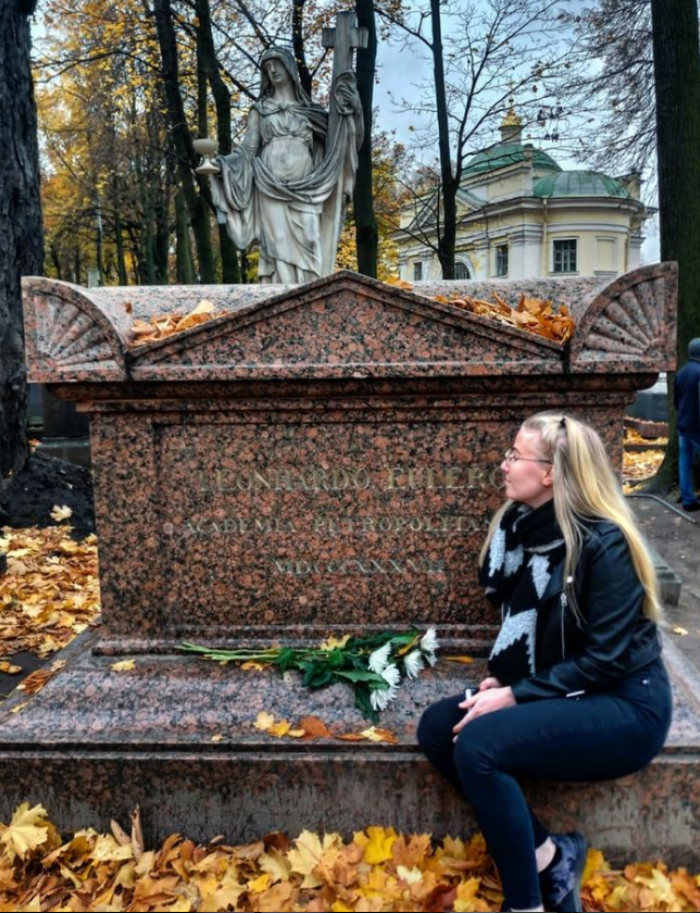
\includegraphics[bb=50 50 300 300,width=0.5\textwidth]{eulerinhauta.png}
    \caption{Eulerin haudalla Pietarissa lokakuussa 2019}
    \label{fig:hauta}
\end{figure}

\section{Eulerin tie lukuteorian pariin}

\section{Merkittävimmät jutut}

%\section{Mitä olisimmekaan ilman Euleria?}

 
\nocite{*}
\printbibliography
 

 
\end{document}